% !TEX root = ./main.tex
% !TEX encoding = UTF-8 Unicode
% !TEX program = pdflatex
% !TeX spellcheck = it_IT

\graphicspath{{Immagini/},{Immagini/webServer/}}

\chapter{Web Server}

\section{Traccia}
Emulare un Web Server Apache ed un set di utenti che richiedono delle risorse.
Monitorare il workload osservato, successivamente caratterizzarlo ed effettuare
un'analisi di performance.\\

\section{Piattaforma}
\subsubsection*{Client}
Il client su cui è stato eseguito \textbf{JMeter}(un generatore di workload), è
un notebook MSI con le seguenti caratteristiche:

\begin{itemize}
  \item \textbf{Processore}: Intel(R) Core(TM) i7-7700HQ @ 2.80GHz
  \item \textbf{Memoria Ram}: 16GB DDR4-2400MHz
  \item \textbf{Tipo sistema}: Windows 10 64bit, processore basato su x64
  \item \textbf{Storage}: SSD Kingston M.2.SATA 480GB
\end{itemize}

\subsubsection*{Server}

Il Web Server Apache è stato installato su un notebook Asus con le seguenti
caratteristiche:

\begin{itemize}
  \item \textbf{Processore}: Intel(R) Core(TM) Pentium
  \item \textbf{Memoria Ram}: 4GB DDR3-1600MHz
  \item \textbf{Tipo sistema}: Ubuntu 16.4 LTS, processore basato su x64
  \item \textbf{Storage}: SSD Samsung 850 EVO SATA 3
\end{itemize}

La connessione Client-Server è stata effettuata in modo diretto tramite un
cavo ethernet.\\

\section{Caratterizzazione Workload}
Per caratterizzare il Workload sono state simulate richieste HTTP random al server,
teli richieste sono state effettuate su 6 pagine html.\\
Le pagine differiscono per dimensione e per tipologia:

\begin{itemize}
  \item Dimensione
  \begin{itemize}
    \item \textbf{\textit{Piccole}}: dell'ordine delle decine di KB;
    \item \textbf{\textit{Medie}}: dell'ordine delle centinaia di KB;
    \item \textbf{\textit{Grandi}}: dell'ordine delle migliaia di KB;
  \end{itemize}
  \item Tipologia
  \begin{itemize}
    \item \textbf{\textit{Testo}};
    \item \textbf{\textit{Immagine}}.
  \end{itemize}
\end{itemize}

Lato Client, i dati sono stati collezionati con il tool \textbf{Jmeter}, configurando
un \textit{Test Plan} opportuno.\\
Lato Server, invece, i dati sono stati collezionati con il tool \textbf{collectl}
di Linux.\\
Il numero di pagine, la dimensione ed il numero di Thread Groups scelti per la
caratterizzazione del workload sono frutto di un'attenta analisi preliminare.\\

\subsection{Problematica Saturazione Server}
Durante gli esperimenti preliminari sostenuti per comprendere al meglio gli strumenti
e i parametri a disposizione, si è giunti alla conclusione che non è possibile,
utilizzando una sola macchina client, saturare al meglio la macchina server.\\
Infatti, in conclusione ai test effettuati, si è dedotto che, prima di riuscire
a saturare le risorse hardware del server, quali CPU e RAM, il collo di bottiglia
è rappresentato dall'infrastruttura di rete.\\
In particolare, il comportamento evidenziatosi è dovuto alla mancata risposta
del Server a tutte le sollecitazioni prodotte dal Client, nonostante
il monitoraggio delle risorse del primo mostrasse di essere ben lontano
dalla sua soglia massima di capacità servente.\\
Nelle seguenti figure sono riportati i report degli esperimenti svolti in JMeter
ed il monitoraggio delle risorse del server, al variare del numero di Thread Group
istanziati.\\

\subsubsection{Esperimento con 10 Thread Group}
 \begin{minipage}{\linewidth}
 	\centering
 	\begin{minipage}{1\linewidth}
 		\begin{figure}[H]
 			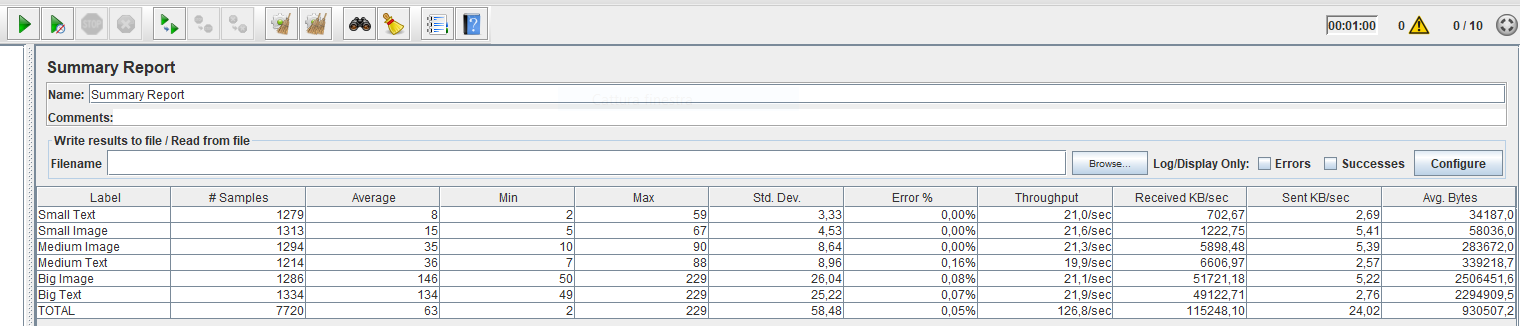
\includegraphics[width=\linewidth]{jmeter_analisi_10thread}
 		\end{figure}
 	\end{minipage}
 	\begin{minipage}{1\linewidth}
 		\begin{figure}[H]
 			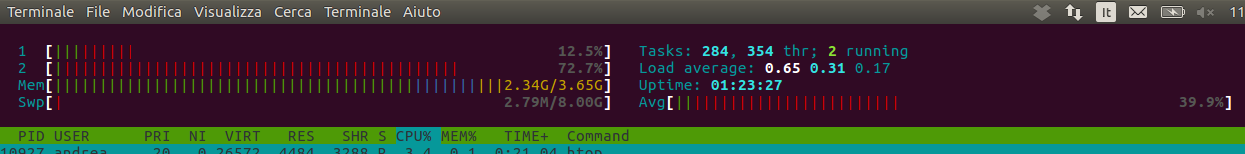
\includegraphics[width=\linewidth]{100_thread_server}
    \end{figure}
  \end{minipage}
\end{minipage}

\subsubsection{Esperimento con 100 Thread Group}
 \begin{minipage}{\linewidth}
 	\centering
 	\begin{minipage}{1\linewidth}
 		\begin{figure}[H]
 			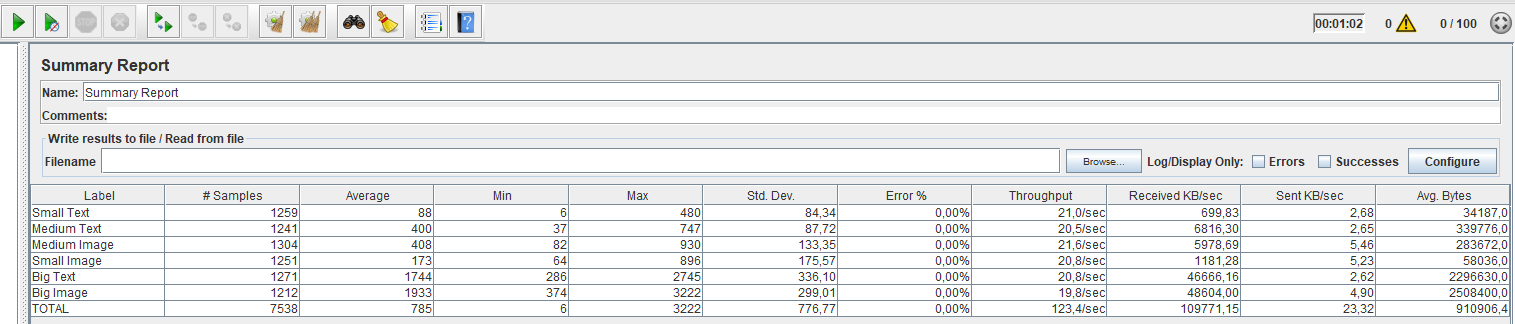
\includegraphics[width=\linewidth]{jmeter_analisi_100thread}
 		\end{figure}
 	\end{minipage}
 	\begin{minipage}{1\linewidth}
 		\begin{figure}[H]
 			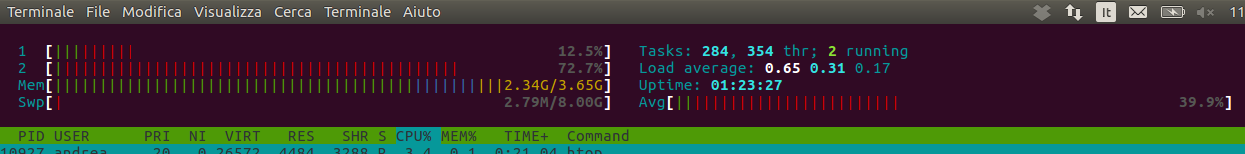
\includegraphics[width=\linewidth]{100_thread_server}
    \end{figure}
  \end{minipage}
\end{minipage}

\subsubsection{Esperimento con 500 Thread Group}
 \begin{minipage}{\linewidth}
 	\centering
 	\begin{minipage}{1\linewidth}
 		\begin{figure}[H]
 			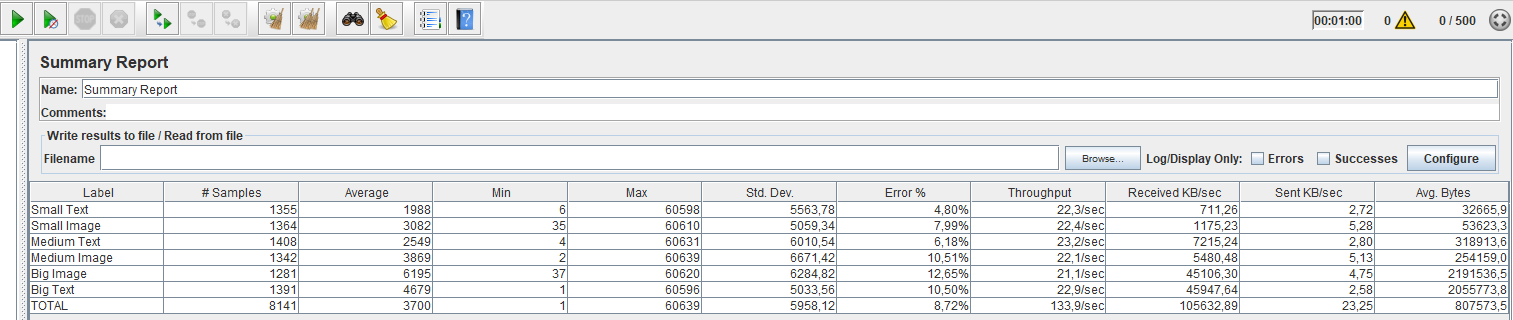
\includegraphics[width=\linewidth]{jmeter_analisi_500thread}
 		\end{figure}
 	\end{minipage}
 	\begin{minipage}{1\linewidth}
 		\begin{figure}[H]
 			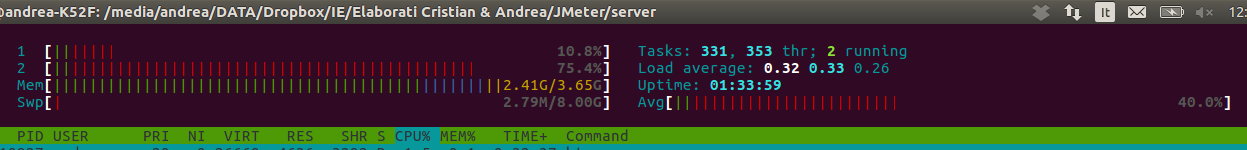
\includegraphics[width=\linewidth]{500_thread_server}
    \end{figure}
  \end{minipage}
\end{minipage}

\subsubsection{Esperimento con 1000 Thread Group}
 \begin{minipage}{\linewidth}
 	\centering
 	\begin{minipage}{1\linewidth}
 		\begin{figure}[H]
 			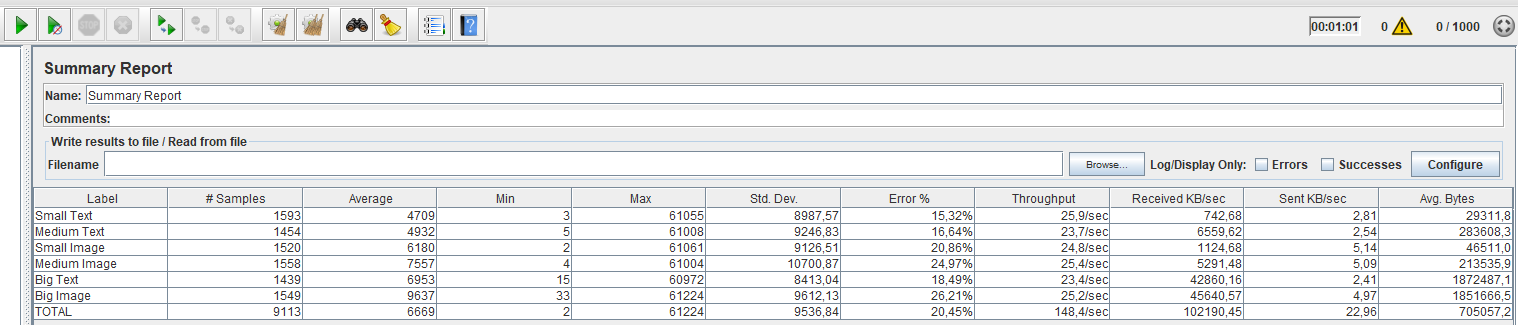
\includegraphics[width=\linewidth]{jmeter_analisi_1000thread}
 		\end{figure}
 	\end{minipage}
 	\begin{minipage}{1\linewidth}
 		\begin{figure}[H]
 			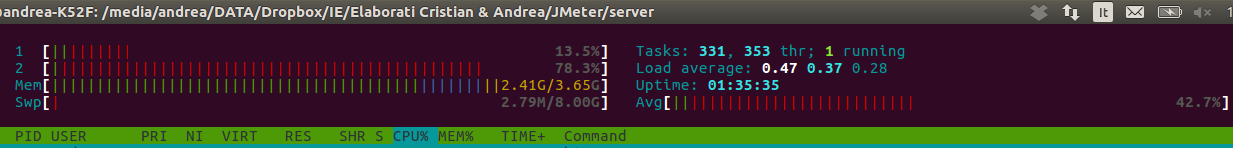
\includegraphics[width=\linewidth]{1000_thread_server}
    \end{figure}
  \end{minipage}
\end{minipage}

\vspace{1cm}
Il parametro Thread Group indica il numero di clients che effettuano continuamente
richieste HTTP al server.\\
Ovviamente questo numero di Threads è simulato dall'unica macchina client utilizzata,
tramite il tool JMeter.\\
Come si può osservare dalle immagini riportate, essendoci una sola macchina fisica,
al crescere del numero di richieste aumenta il numero di errori.\\
Questi errori però non sono da individuare nell'incapacità del server di gestire
la mole di richieste(infatti la CPU è mediamente occupata a circa il 40\% mentre
la RAM al 65\%), bensì nell'infrastruttura di rete(scheda di rete e cavo Ethernet),
limitata ad \textbf{1Gb/s}.\\

In \figurename~\ref{bottleneck_rete} è riportato l'utilizzo dell'I/O di rete,
raffigurante, in alcuni punti, il raggiungimento del limite fisico(1Gb/s).\\
\begin{figure}[!htbp]
  \centering
  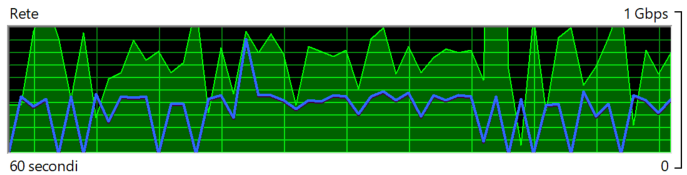
\includegraphics[width=1\linewidth, keepaspectratio]{client_rete_bottleneck}
  \caption{Infrastruttura di Rete - Bottleneck}
  \label{bottleneck_rete}
\end{figure}

\clearpage

\subsection{Analisi Alto Livello (Client)}
\subsubsection*{Impostazioni Client (JMeter)}
Prima di effettuare gli esperimenti, è stato necessario configurare alcuni parametri
nel Test Plan di JMeter, riportati in \figurename~\ref{conf_jmeter}

\begin{figure}[!htbp]
  \centering
  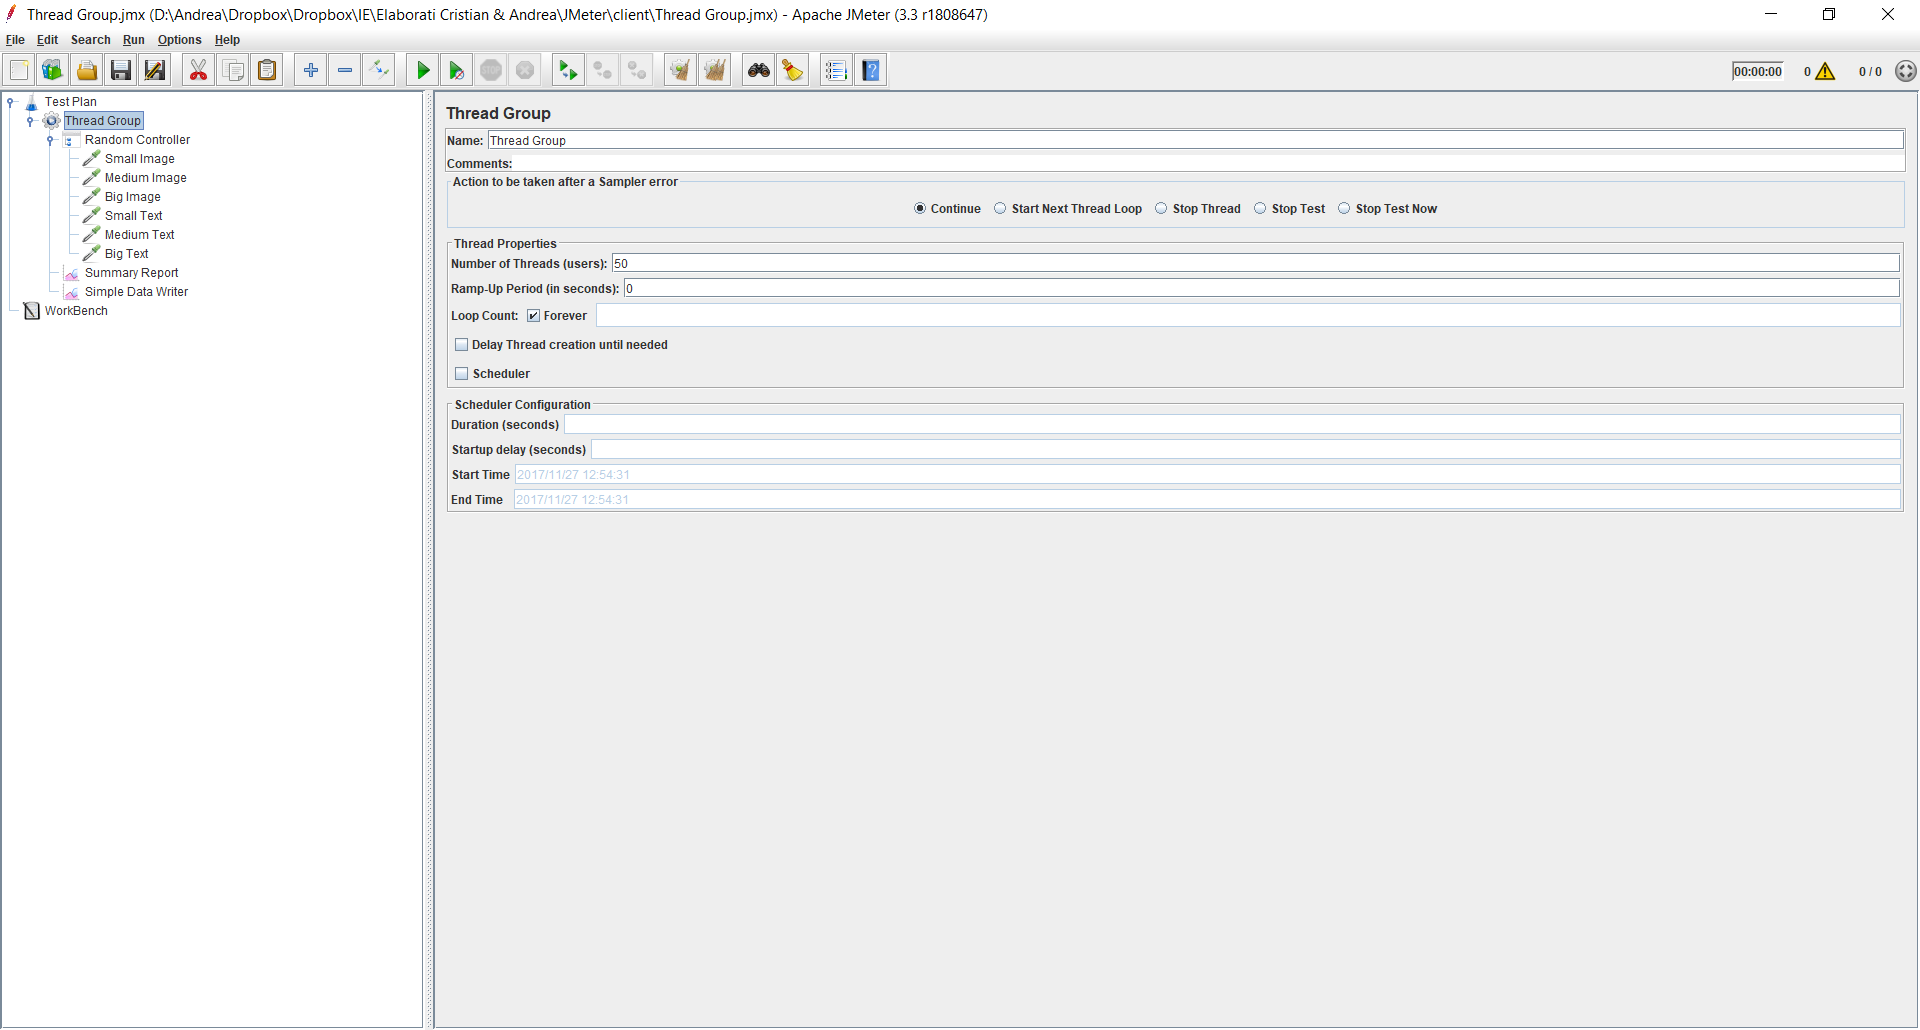
\includegraphics[width=1\linewidth, keepaspectratio]{conf_thread_group}
  \caption{}
  \label{conf_jmeter}
\end{figure}

In particolare, si evince che il Test Plan è stato caratterizzato dai seguenti
componenti:

\begin{itemize}
  \item \textbf{\textit{Random Controller}} - per generare richieste tra le possibili
  pagine in maniera randomica ed uniforme;
  \item \textbf{\textit{HTTP Request}} - una per pagina, serve per generare una
  richiesta HTTP;
  \item \textbf{\textit{Summary Report}} - genera un report immediato degli esperimenti
  in esecuzione.
  \item \textbf{\textit{Simple Data Writer}} - scrive i risultati degli esperimenti
  in un file .csv
\end{itemize}

JMeter è stato configurato attivando il \textbf{Keep Alive} ad ogni pagina
ed il parametro \textbf{Retrieve All Embedded Resources}(necessario per prelevare
le immagini linkate nell'html).\\
Nonostante gli esperimenti siano stati eseguiti per un tempo di 8 minuti, è stato
effettuato un filtraggio dei dati del primo ed ultimo minuto di esecuzione, al fine
di eliminare eventuali comportamenti transitivi.\\

I parametri utilizzati per la caratterizzazione del workload lato client sono:
\textbf{Latency}, \textbf{Elapsed Time}, \textbf{Bytes}.\\

In \figurename~\ref{distribuzioni_parametri} sono riportate le distribuzioni dei
tre parametri.\\

\begin{figure}[!htbp]
  \centering
  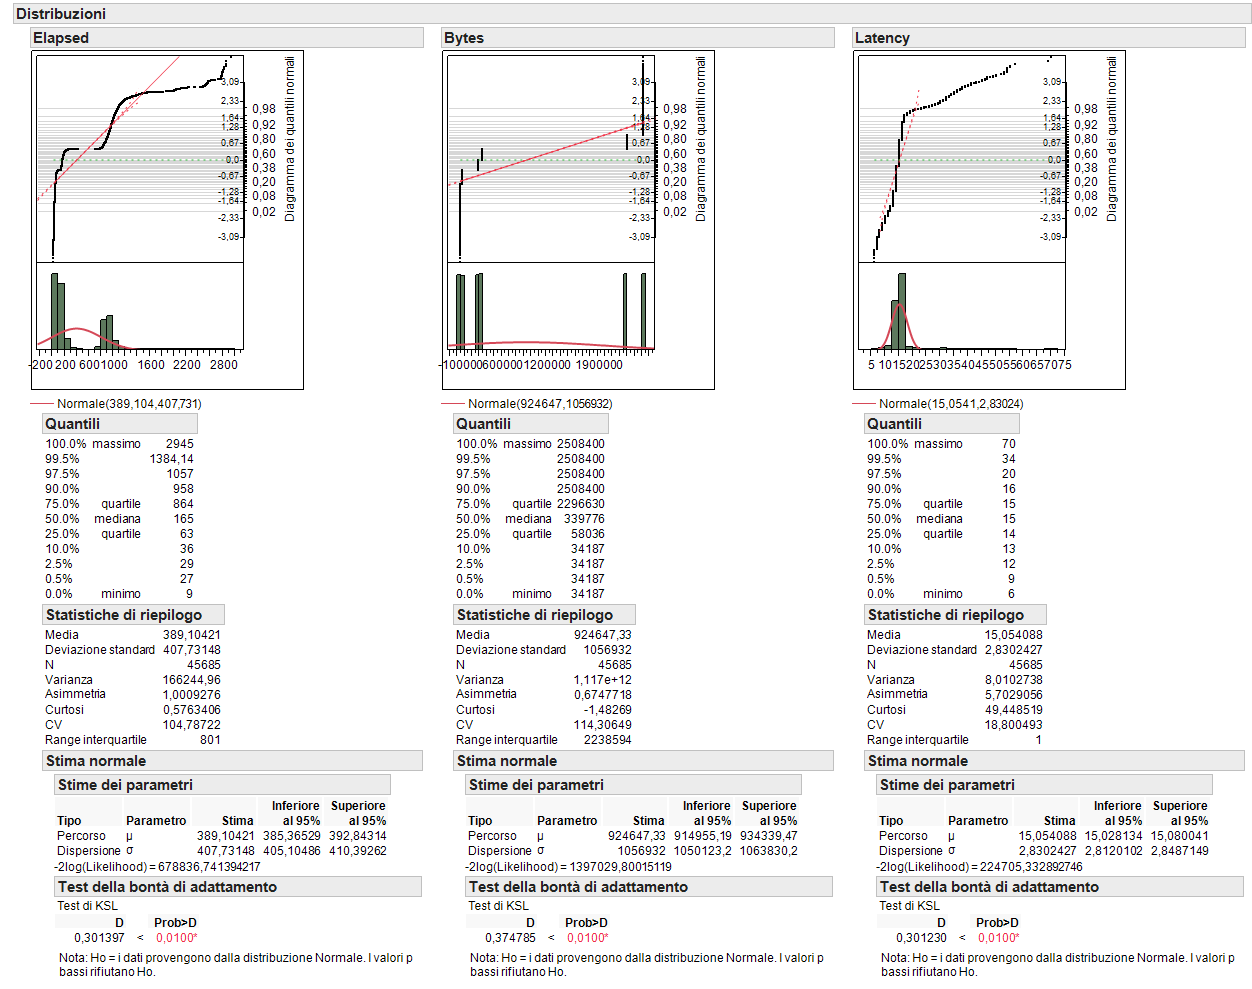
\includegraphics[width=1\linewidth, keepaspectratio]{distribuzioni_client}
  \caption{}
  \label{distribuzioni_parametri}
\end{figure}

Come si può osservare dal plot Q-Q e dal test di bontà di adattamento, le distribuzioni
non sono normali, di conseguenza, si scelgono \textit{mediana}, come indice di
tendenza centrale e \textit{SIQR}, come indice di dispersione.\\

\begin{center}
	\begin{tabular}{c|c|c|c|}
		& \textbf{Latency} & \textbf{Elapsed Time} & \textbf{Bytes} \\
		\hline
		\textbf{Mediana} & 15 & 165 & 339776 \\
		\hline
		\textbf{SIQR} & 1 & 801 & 2238594 \\
		\hline
	\end{tabular}
\end{center}

\subsubsection*{Correlazione Parametri}
Nella seguente fase vengono studiate possibili correlazioni presenti tra i tre
parametri considerati.\\
Per studiare la correlazione, non volendo fare assunzioni sulla natura delle
distribuzioni, è possibile svolgere il test non parametrico di \textbf{Kendall}.\\
Tale test assume come ipotesi nulla l'indipendenza dei fattori.\\
In particolare, si è interessati ad osservare eventuali correlazioni tra la Latency
e l'Elapsed Time, in \figurename~\ref{correlazione_elapsed_latency}.\\
\begin{figure}[!htbp]
  \centering
  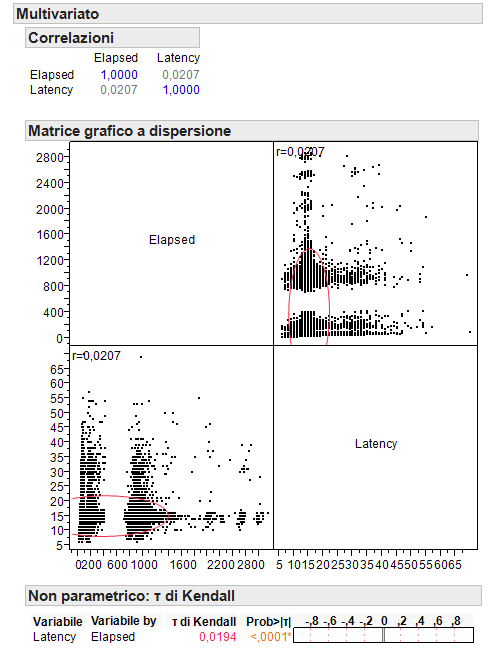
\includegraphics[width=.7\linewidth, keepaspectratio]{correlazione_elapsed_latency}
  \caption{}
  \label{correlazione_elapsed_latency}
\end{figure}

In questo caso, il test di Kendall suggerisce che l'ipotesi di indipendenza è
rigettata, quindi esiste una forte dipendenza tra i parametri \textit{Latency} e
\textit{Elapsed Time}.\\
